\documentclass{standalone}
\usepackage{pgfplots}
\begin{document}
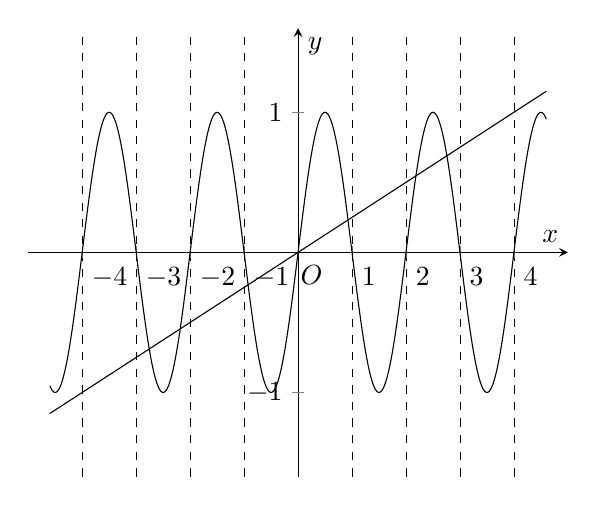
\begin{tikzpicture}
\begin{axis}
[
ymin=-1.6,ymax=1.6,
xmin=-5,xmax=5,
xtick=\empty,
ytick=\empty,
extra x ticks={-4, -3, -2, -1, 1, 2, 3, 4},
extra x tick labels={$-4$, $-3$, $-2$, $-1$, $1$, $2$, $3$, $4$},
extra y ticks={-1, 1},
extra y tick labels={$-1$, $1$},
every extra x tick/.style={
    xticklabel style={anchor=north west},
    grid=major,
    major grid style={very thin,dashed,black}
},
axis lines = center,
xlabel=$x$,ylabel=$y$,
samples=200,
]
\addplot [black, domain=-4.6:4.6, samples=400] {sin(deg(pi*x))};
\addplot [black, domain=-4.6:4.6] {x/4};
\node at (axis cs:0.25, -0.16) {$O$} ;
\end{axis}
\end{tikzpicture}
\end{document}
